% Options for packages loaded elsewhere
\PassOptionsToPackage{unicode}{hyperref}
\PassOptionsToPackage{hyphens}{url}
%
\documentclass[
  letterpaper,
  ignorenonframetext,
  aspectratio=43,
  handout,
  12pt]{beamer}
\usepackage{pgfpages}
\setbeamertemplate{caption}[numbered]
\setbeamertemplate{caption label separator}{: }
\setbeamercolor{caption name}{fg=normal text.fg}
\beamertemplatenavigationsymbolsempty
% Prevent slide breaks in the middle of a paragraph
\widowpenalties 1 10000
\raggedbottom
\setbeamertemplate{part page}{
  \centering
  \begin{beamercolorbox}[sep=16pt,center]{part title}
    \usebeamerfont{part title}\insertpart\par
  \end{beamercolorbox}
}
\setbeamertemplate{section page}{
  \centering
  \begin{beamercolorbox}[sep=12pt,center]{part title}
    \usebeamerfont{section title}\insertsection\par
  \end{beamercolorbox}
}
\setbeamertemplate{subsection page}{
  \centering
  \begin{beamercolorbox}[sep=8pt,center]{part title}
    \usebeamerfont{subsection title}\insertsubsection\par
  \end{beamercolorbox}
}
\AtBeginPart{
  \frame{\partpage}
}
\AtBeginSection{
  \ifbibliography
  \else
    \frame{\sectionpage}
  \fi
}
\AtBeginSubsection{
  \frame{\subsectionpage}
}
\usepackage{amsmath,amssymb}
\usepackage{lmodern}
\usepackage{ifxetex,ifluatex}
\ifnum 0\ifxetex 1\fi\ifluatex 1\fi=0 % if pdftex
  \usepackage[T1]{fontenc}
  \usepackage[utf8]{inputenc}
  \usepackage{textcomp} % provide euro and other symbols
\else % if luatex or xetex
  \usepackage{unicode-math}
  \defaultfontfeatures{Scale=MatchLowercase}
  \defaultfontfeatures[\rmfamily]{Ligatures=TeX,Scale=1}
\fi
\usetheme[]{metropolis}
% Use upquote if available, for straight quotes in verbatim environments
\IfFileExists{upquote.sty}{\usepackage{upquote}}{}
\IfFileExists{microtype.sty}{% use microtype if available
  \usepackage[]{microtype}
  \UseMicrotypeSet[protrusion]{basicmath} % disable protrusion for tt fonts
}{}
\makeatletter
\@ifundefined{KOMAClassName}{% if non-KOMA class
  \IfFileExists{parskip.sty}{%
    \usepackage{parskip}
  }{% else
    \setlength{\parindent}{0pt}
    \setlength{\parskip}{6pt plus 2pt minus 1pt}}
}{% if KOMA class
  \KOMAoptions{parskip=half}}
\makeatother
\usepackage{xcolor}
\IfFileExists{xurl.sty}{\usepackage{xurl}}{} % add URL line breaks if available
\IfFileExists{bookmark.sty}{\usepackage{bookmark}}{\usepackage{hyperref}}
\hypersetup{
  hidelinks,
  pdfcreator={LaTeX via pandoc}}
\urlstyle{same} % disable monospaced font for URLs
\newif\ifbibliography
\usepackage{graphicx}
\makeatletter
\def\maxwidth{\ifdim\Gin@nat@width>\linewidth\linewidth\else\Gin@nat@width\fi}
\def\maxheight{\ifdim\Gin@nat@height>\textheight\textheight\else\Gin@nat@height\fi}
\makeatother
% Scale images if necessary, so that they will not overflow the page
% margins by default, and it is still possible to overwrite the defaults
% using explicit options in \includegraphics[width, height, ...]{}
\setkeys{Gin}{width=\maxwidth,height=\maxheight,keepaspectratio}
% Set default figure placement to htbp
\makeatletter
\def\fps@figure{htbp}
\makeatother
% Make links footnotes instead of hotlinks:
\DeclareRobustCommand{\href}[2]{#2\footnote{\url{#1}}}
\setlength{\emergencystretch}{3em} % prevent overfull lines
\providecommand{\tightlist}{%
  \setlength{\itemsep}{0pt}\setlength{\parskip}{0pt}}
\setcounter{secnumdepth}{-\maxdimen} % remove section numbering
\usepackage{pgfpages}
\pgfpagesuselayout{2 on 1}
\providecommand{\tightlist}{%
\setlength{\itemsep}{0pt}\setlength{\parskip}{0pt}}
\makeatletter
\makeatother
\let\Oldincludegraphics\includegraphics
\renewcommand{\includegraphics}[2][]{\Oldincludegraphics[width=\textwidth,height=0.7\textheight,keepaspectratio]{#2}}
\ifluatex
  \usepackage{selnolig}  % disable illegal ligatures
\fi

\author{}
\date{}

\begin{document}

\begin{frame}{Mechanics of Materials}
\protect\hypertarget{mechanics-of-materials}{}
Lecture 5 - Axial Load

Dr.~Nicholas Smith

Wichita State University, Department of Aerospace Engineering

February 15, 2021
\end{frame}

\begin{frame}{schedule}
\protect\hypertarget{schedule}{}
\begin{itemize}
\tightlist
\item
  15 Feb - Axial Load (not on exam 1)
\item
  17 Feb - Exam Review
\item
  19 Feb - Homework 2 Due, Homework 1 Self-grade Due
\item
  22 Feb - Exam 1
\item
  26 Feb - Project 1 Due
\end{itemize}
\end{frame}

\begin{frame}{outline}
\protect\hypertarget{outline}{}
\begin{itemize}
\tightlist
\item
  saint venant's principle
\item
  elastic axial deformation
\item
  superposition
\item
  statically indeterminate
\end{itemize}
\end{frame}

\hypertarget{saint-venants-principle}{%
\section{saint venant's principle}\label{saint-venants-principle}}

\begin{frame}{saint venant's principle}
\protect\hypertarget{saint-venants-principle-1}{}
\begin{itemize}
\tightlist
\item
  We use Saint Venant's principle to generalize various loading
  applications
\item
  If we apply a concentrated force, near where we apply it (for example,
  along a pin), the stress will not be very uniform
\item
  Far away from that point, however, the stress will be uniform, whether
  we apply the force with 1 pin, 2 pins, or via a uniform grip
\end{itemize}
\end{frame}

\begin{frame}{saint venant's principle}
\protect\hypertarget{saint-venants-principle-2}{}
\begin{itemize}
\tightlist
\item
  We use \emph{saint venant's principle} to replace difficult to model
  loads with easier ones
\item
  There are two conditions

  \begin{enumerate}
  \tightlist
  \item
    The load must be statically equivalent
  \item
    Our region of interest must be far enough away from the point where
    the load was applied
  \end{enumerate}
\end{itemize}
\end{frame}

\begin{frame}{saint venant's principle}
\protect\hypertarget{saint-venants-principle-3}{}
\begin{figure}
\centering
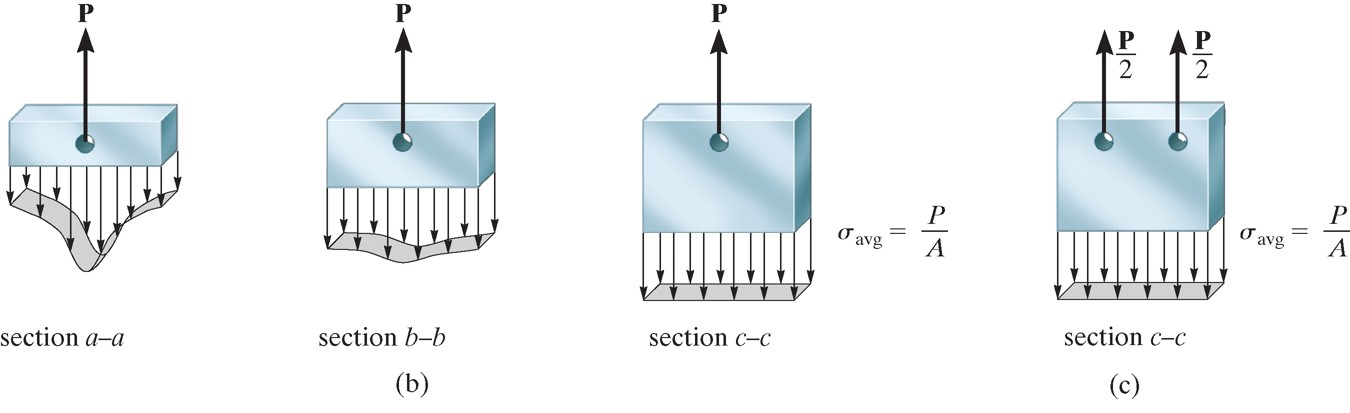
\includegraphics{../images/st-venant.jpg}
\caption{An image showing what the stress field looks like in a body
both near to an applied load and far away.}
\end{figure}
\end{frame}

\hypertarget{elastic-axial-deformation}{%
\section{elastic axial deformation}\label{elastic-axial-deformation}}

\begin{frame}{axially loaded member}
\protect\hypertarget{axially-loaded-member}{}
\begin{itemize}
\tightlist
\item
  We can use Hooke's Law to find the deformation of a general body under
  axial loading (below the elastic limit)
\end{itemize}

\begin{figure}
\centering
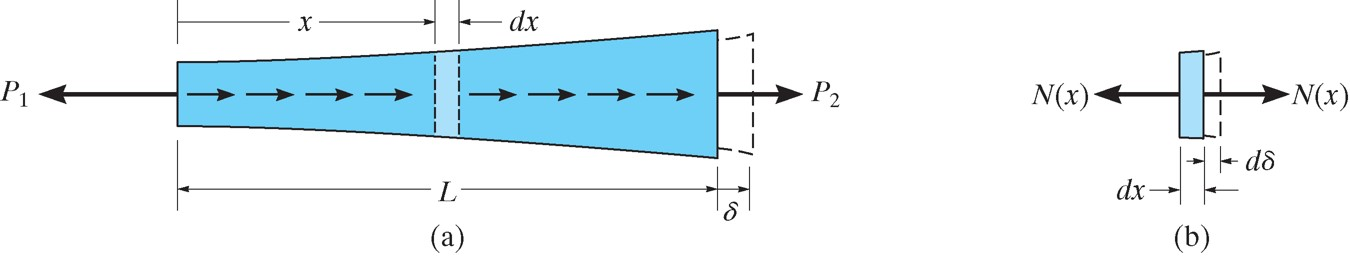
\includegraphics{../images/axial-load.jpg}
\caption{If we consider some homogeneous body with an applied load, we
can look at a small section of this body with an applied load of N(x)
which is initially dx wide, but under load stretches an additional d
delta.}
\end{figure}
\end{frame}

\begin{frame}{axially loaded member}
\protect\hypertarget{axially-loaded-member-1}{}
\begin{itemize}
\tightlist
\item
  For some differential element, we can consider the internal forces and
  stresses
\end{itemize}

\[\sigma = \frac{N(x)}{A(x)} = E(x) \epsilon(x) = E(x) \left(\frac{d\delta}{dx}\right)\]

\begin{itemize}
\tightlist
\item
  We can solve this for \(d\delta\) to find
\end{itemize}

\[d \delta = \frac{N(x) dx}{A(x)E(x)}\]

\begin{itemize}
\tightlist
\item
  We integrate this over the length of the bar to find the total
  displacement
\end{itemize}
\end{frame}

\begin{frame}{sign convention}
\protect\hypertarget{sign-convention}{}
\begin{itemize}
\tightlist
\item
  In general, we consider a force or stress to be positive if it causes
  tension and elongation
\item
  It is negative if it causes compression and contraction
\end{itemize}
\end{frame}

\begin{frame}{example 4.2}
\protect\hypertarget{example-4.2}{}
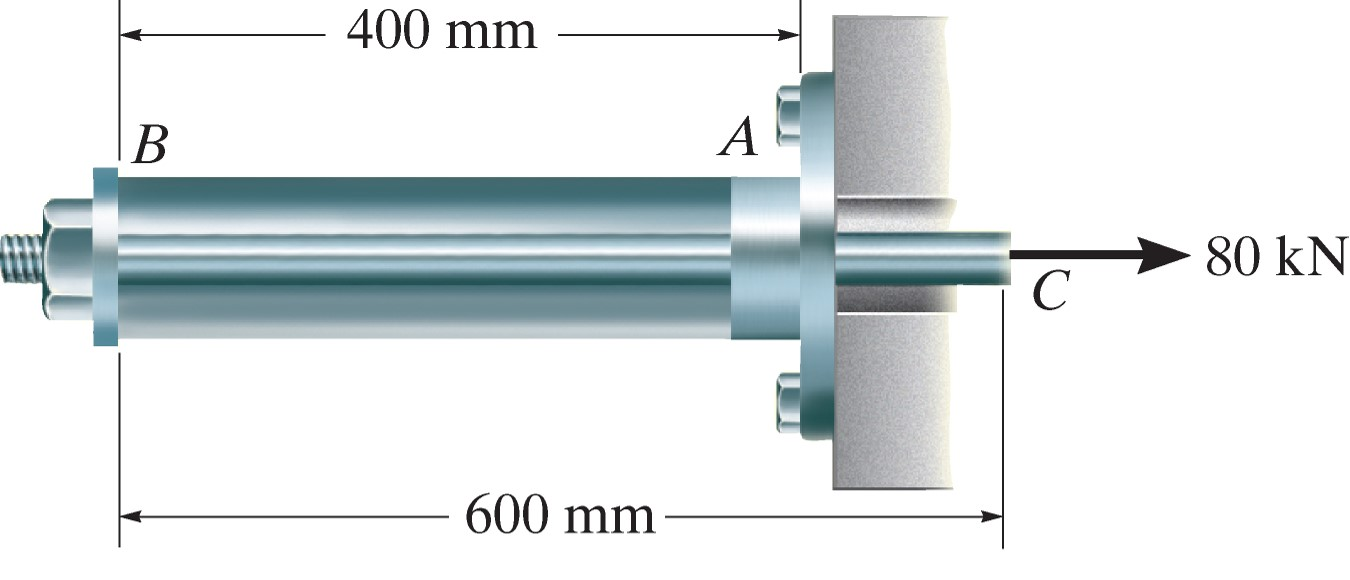
\includegraphics{../images/example-4-2.jpg}

A steel rod with a 10mm diameter is attached to a rigid collar passing
through an aluminum tube with cross-sectional area of 400 mm2. Find the
displacement at C if \(E_{st} = 200\) GPa and \(E_{al} = 70\) GPa.
\end{frame}

\begin{frame}{example 4.4}
\protect\hypertarget{example-4.4}{}
:::::::::::::: \{.columns\} ::: \{.column width=``50\%''\}
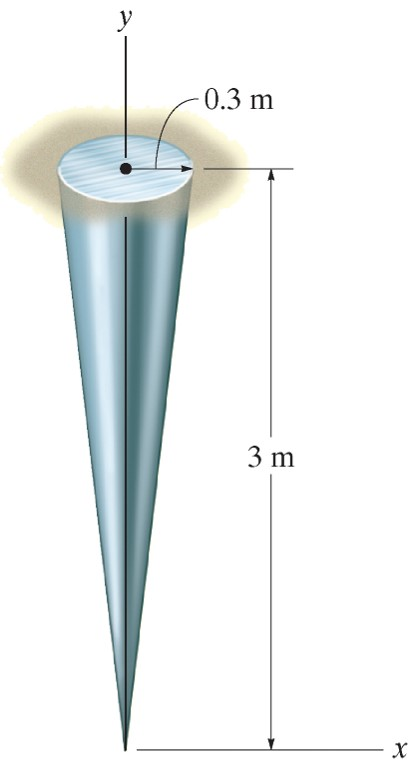
\includegraphics{../images/example-4-4.jpg}

\begin{column}{0.5\textwidth}
The cone shown has a specific weight of \(\gamma = 6\) kN/m3 and E=9
GPa. Determine how far the end is displaced due to gravity.
\end{column}

::::::::::::::
\end{frame}

\hypertarget{superposition}{%
\section{superposition}\label{superposition}}

\begin{frame}{superposition}
\protect\hypertarget{superposition-1}{}
\begin{itemize}
\tightlist
\item
  Some problems are too complicated to solve all at once
\item
  Instead, we break them up into two simpler problems
\item
  Each ``sub-problem'' must still satisfy equilibrium
\item
  Problem must be linear and the deformation should be small enough that
  it does not cause moment-equilibrium issues
\end{itemize}
\end{frame}

\hypertarget{statically-indeterminate}{%
\section{statically indeterminate}\label{statically-indeterminate}}

\begin{frame}{statically indeterminate}
\protect\hypertarget{statically-indeterminate-1}{}
\begin{itemize}
\tightlist
\item
  There are many problems that are at least slightly over-constrained
\item
  While this is common engineering practice, it creates too many
  variables for statics analysis
\item
  These problems are called ``statically indeterminate''
\end{itemize}
\end{frame}

\begin{frame}{statically indeterminate}
\protect\hypertarget{statically-indeterminate-2}{}
\begin{itemize}
\tightlist
\item
  One extra equation we can use is called ``compatibility'' or the
  ``kinematic condition''
\item
  We know that at the displacement must be equal on both sides of any
  arbitrary section we make in a member
\item
  We can separate a member into two parts, then use compatibility to
  relate the two unknown forces
\end{itemize}
\end{frame}

\begin{frame}{statically indeterminate}
\protect\hypertarget{statically-indeterminate-3}{}
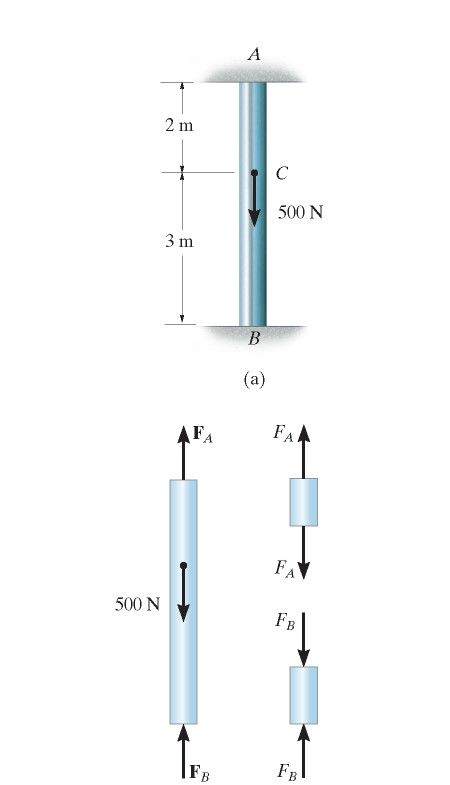
\includegraphics{../images/statically-indeterminate.jpg}
\end{frame}

\begin{frame}{example 4.7}
\protect\hypertarget{example-4.7}{}
\begin{columns}[T]
\begin{column}{0.5\textwidth}
\begin{figure}
\centering
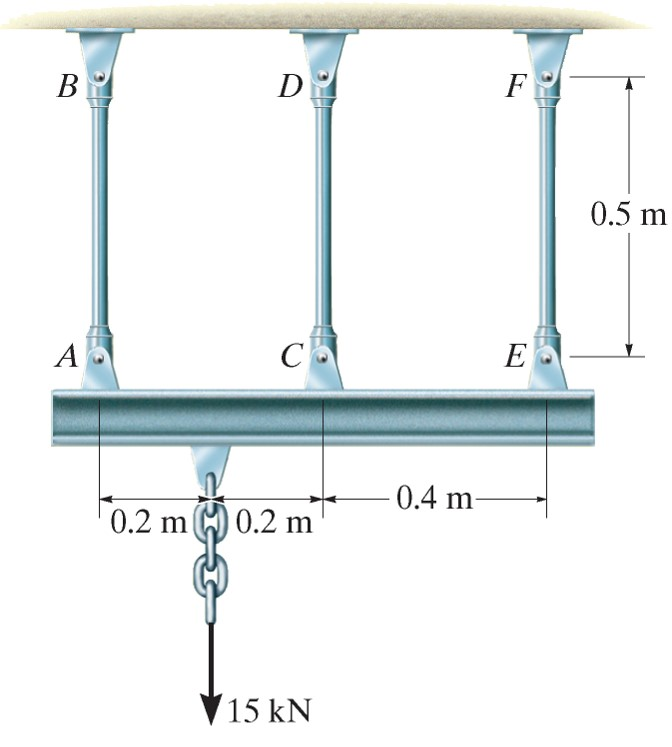
\includegraphics{../images/example-4-7.jpg}
\caption{A 0.8 m long rigid horizontal bar is supported by hanging from
3 vertical rods. Rod AB supports the left end, rod CD supports the
middle and rod EF supports the right end. A 15 kN load is applied 0.2 m
from the left end.}
\end{figure}
\end{column}

\begin{column}{0.5\textwidth}
Assuming the bottom bar is rigid, find the force developed in each bar.
AB and EF have cross-sectional areas of 50 mm2 while CD has a
cross-sectional area of 30 mm2.
\end{column}
\end{columns}
\end{frame}

\end{document}
